\documentclass[UTF8,oneside]{ctexbook}

\usepackage[titles]{tocloft} % 目录
\usepackage[colorlinks,linkcolor=blue]{hyperref} % 超链接
\usepackage{graphicx} % An example of a floating figure using the graphicx package.
\usepackage{animate} % 动画
\usepackage{enumerate} % 列表
\usepackage{fancyhdr} % 页眉页脚
\pagestyle{fancy}
\usepackage{xpinyin} % 注音
\usepackage[]{appendix}

\title{\Huge{A NOTE {\itshape of} MASTER}\\
\Huge{菜鸟硕士手册}\\
\large{V1.0}}
\author{\href{https://github.com/lonelybag?tab=repositories}{\Large{@LonelyBag}}\\ {\itshape \large{Edite by \href{https://mirrors.tuna.tsinghua.edu.cn/CTAN/systems/texlive/Images/}{\LaTeX}}}}

\begin{document}
% ----------- 封面 ---------------
\frontmatter
\maketitle

% \begin{center}  % 居中
% 	\quad \\
% 	\vspace{3cm}
% 	\hspace{3cm}\Huge{A NOTE {\itshape of} MASTER}\\
% 	\hspace{3cm}\Huge{菜鸟硕士手册} \\
% 	\hspace{3cm}\large{V1.0} \\
% 	\vspace{5cm}
% 	\hspace{3cm}\href{https://github.com/lonelybag/Latex_lonelybag}{\Large{@LonelyBag}}\\
% 	\vspace{0.5cm}
% 	\hspace{3cm}\Large{2018.3.2}
% 	\clearpage  % 清除当页页码
% \end{center}

\begin{center}  % 居中
	\quad \\
	\vspace{5cm}
	\LARGE{如果说我比别人看得更远,那是因为我站在巨人的肩膀上}\\
	% \LARGE{上下四方曰宇,古往今来曰宙}
\end{center}
\thispagestyle{empty}
% ----------- 目录 ---------------
\tableofcontents

\mainmatter
% ----------- 正文 ---------------
\chapter{试着不虚此行}
《千与千寻》中有这样一句话:“人生就是一列开往坟墓的列车,路途上会有很多站,很难有人可以自始至终陪着走完。当陪你的人要下车时,即使不舍也该心存感激,然后挥手道别”。
研究生的学习生涯其实就是人生中的一小段旅程,虽然我们很难提前确定这段火车经过的景色是否是美好的(甚至连经历过的前辈也不能告诉我们,因为每个人的认知与理解都是不同的),但有一点是确定的,那就是当初踏上这段旅程时,我们对未来旅途的兴奋与憧憬。

虽然我不认为会有在读期间的研究生认为自己享受这段时光的,但更加值得注意的是,我也几乎没有听说毕业后的研究生对这段经历表示过后悔。这一事实足以表明,不论你现在经历了什么,一旦你坚持下来,那么这段经历必将让你获得身体和心智的全面提升。换句话说,这是一段极具性价比的人生经历。况且,当初踏上这班列车是我们自己的选择,所以请试着不虚此行。

\section{假如重新来过}
假如我回到了三年前再次读研,可能我会这样度过:
\begin{itemize}
	\item 研一上,认真学好数值分析、矩阵论、智能控制理论、电力电子、DSP以及文献检索(比较有代表性的,不代表其他不重要)。原因:数值分析和矩阵论是一切仿真软件内核的数学基础;智能控制理论涉及到了人工神经网络的基本原理,而它是未来的必然趋势,此外书中提到的算法都可以解决优化问题,如:电路拓扑的构建、电路元件参数的调整、线圈形状的优化等等。。。电力电子电路和DSP的结合是除了仿真外验证思路的最优实现方案;文献检索,可能是硕士期间最重要、也最值得花时间研究的课。
	\item 研一下,系统地学习MATLAB+Simulink、COMSOL或Ansys、DSP、Altium Designer、ADS或Multism、Latex+git+vscode、Rhino或3DSMAX或C4D、PS或Adobe Illustrator。此外,整理近两年的论文。
	\item 研二上(开题10月底),精进MATLAB+Simulink、COMSOL或Ansys、DSP、Altium Designer、ADS或Multism、Latex+git+vscode,并着手仿真实验+写论文引言。
	\item 研二下(中期5月底),完成实验,完成论文并在11月份前投出。
	\item 研二上,着手第二篇论文,在9月份前投出。
	\item 研三上(毕业答辩次年1月底),完成毕业论文。
\end{itemize}

这确实是异常\xpinyin{丰}{tong4}\xpinyin{富}{ku3}的经历,如果坚持下来,你的人生可能就会因此\xpinyin{改}{tu1}\xpinyin{变}{ding3}。

\section{一些感悟}
在这里列举一些自己的感悟。如果能够重新读研,我希望有人告诉我这些事情。
\begin{itemize}
	\item 人生没有输赢,只有选择
	\item 评判一个人的行为,需要结合他的选择
	\item 不要和他人比较,你要赢的只是你自己
	\item 找到自己的兴趣点比找到学习的方法更重要
	\item 掌握学习的方法比掌握一件事物本身更重要
	\item 讨论事情的合理性比完成它更重要
	\item 合理的团队架构比个人的能力更重要
	\item 生活比工作更重要
	\item 生命比生活更重要
	\item 梦想比生命更重要
\end{itemize}

\section{关于本文档的一些解释}
\begin{itemize}
	\item 首先学一个快捷键:Alt+左箭头,用于点击超链接后回退原位置(试试跳到附录\ref{fuluA}再跳回来)
	\item 希望发现问题或者想要补充信息的读者在\href{https://github.com/lonelybag/Latex_lonelybag/issues}{这里}添加issue,帮助我完善这个工具书(需要先注册\href{https://github.com}{Github}账号)
	\item 如果有兴趣,请跟我一起完善\href{https://github.com/lonelybag/MATLAB_DEMO}{MATLAB项目}以及\href{https://github.com/lonelybag/Comsol_lonelybag}{COMSOL项目}
	\item 本文档倾向于仿真与科技论文写作
	\item 本文档由\LaTeX 编辑而成,没有用word的理由是word无法用git进行版本管理
	\item 本文档的内容来源于硕士期间的积累和感悟
	\item 撰写本文档纯属个人兴趣,我不保证对它所造成的任何损失负责
	\item 本文档按照科研(寻找问题 - 确定研究方法 - 提出解决方法 - 获取实验数据 - 分析处理数据 - 发表成果)的一般流程进行撰写
	\item 本文档的意义在于给予启发,而不在于给定一条“路线”
\end{itemize}

\chapter{罗马是如何建成的}
\section{是时候学点管理学了}
\subsection{什么是工作流}
我平常接触github比较多(一个著名的代码托管网站,这是\href{https://github.com/lonelybag?tab=repositories}{我的主页})。我发现,在进行大多数的代码项目前,大家都会提到一个叫做workflow(可以翻译为工作流)的东西。经过了解后,我发现这个东西非常强大,其本质就是所谓的“思路”或者“技术路线”,并且除了给出方法论以外,它还告诉了我们如何进行团队协作。

workflow源于Github,因此先对Github进行介绍。Github由Linus Torvalds编写的版本控制工具Git发展而来,这两样工具的发明最初仅是为了服务于\href{https://github.com/torvalds/linux}{Linux}项目的开发。Linux作为一个操作系统内核,一个人不可能进行维护,而Github的出现,使得世界范围的代码爱好者可以共同维护一个项目,而这在以前是绝无可能的。

如果说Github提供了一个巨型的合作平台,那么workflow则提供了开发者们共同协作的机制。一个典型的github workflow如图\ref{fig:workflow}所示。

\begin{figure}[!htb]
	\centering
	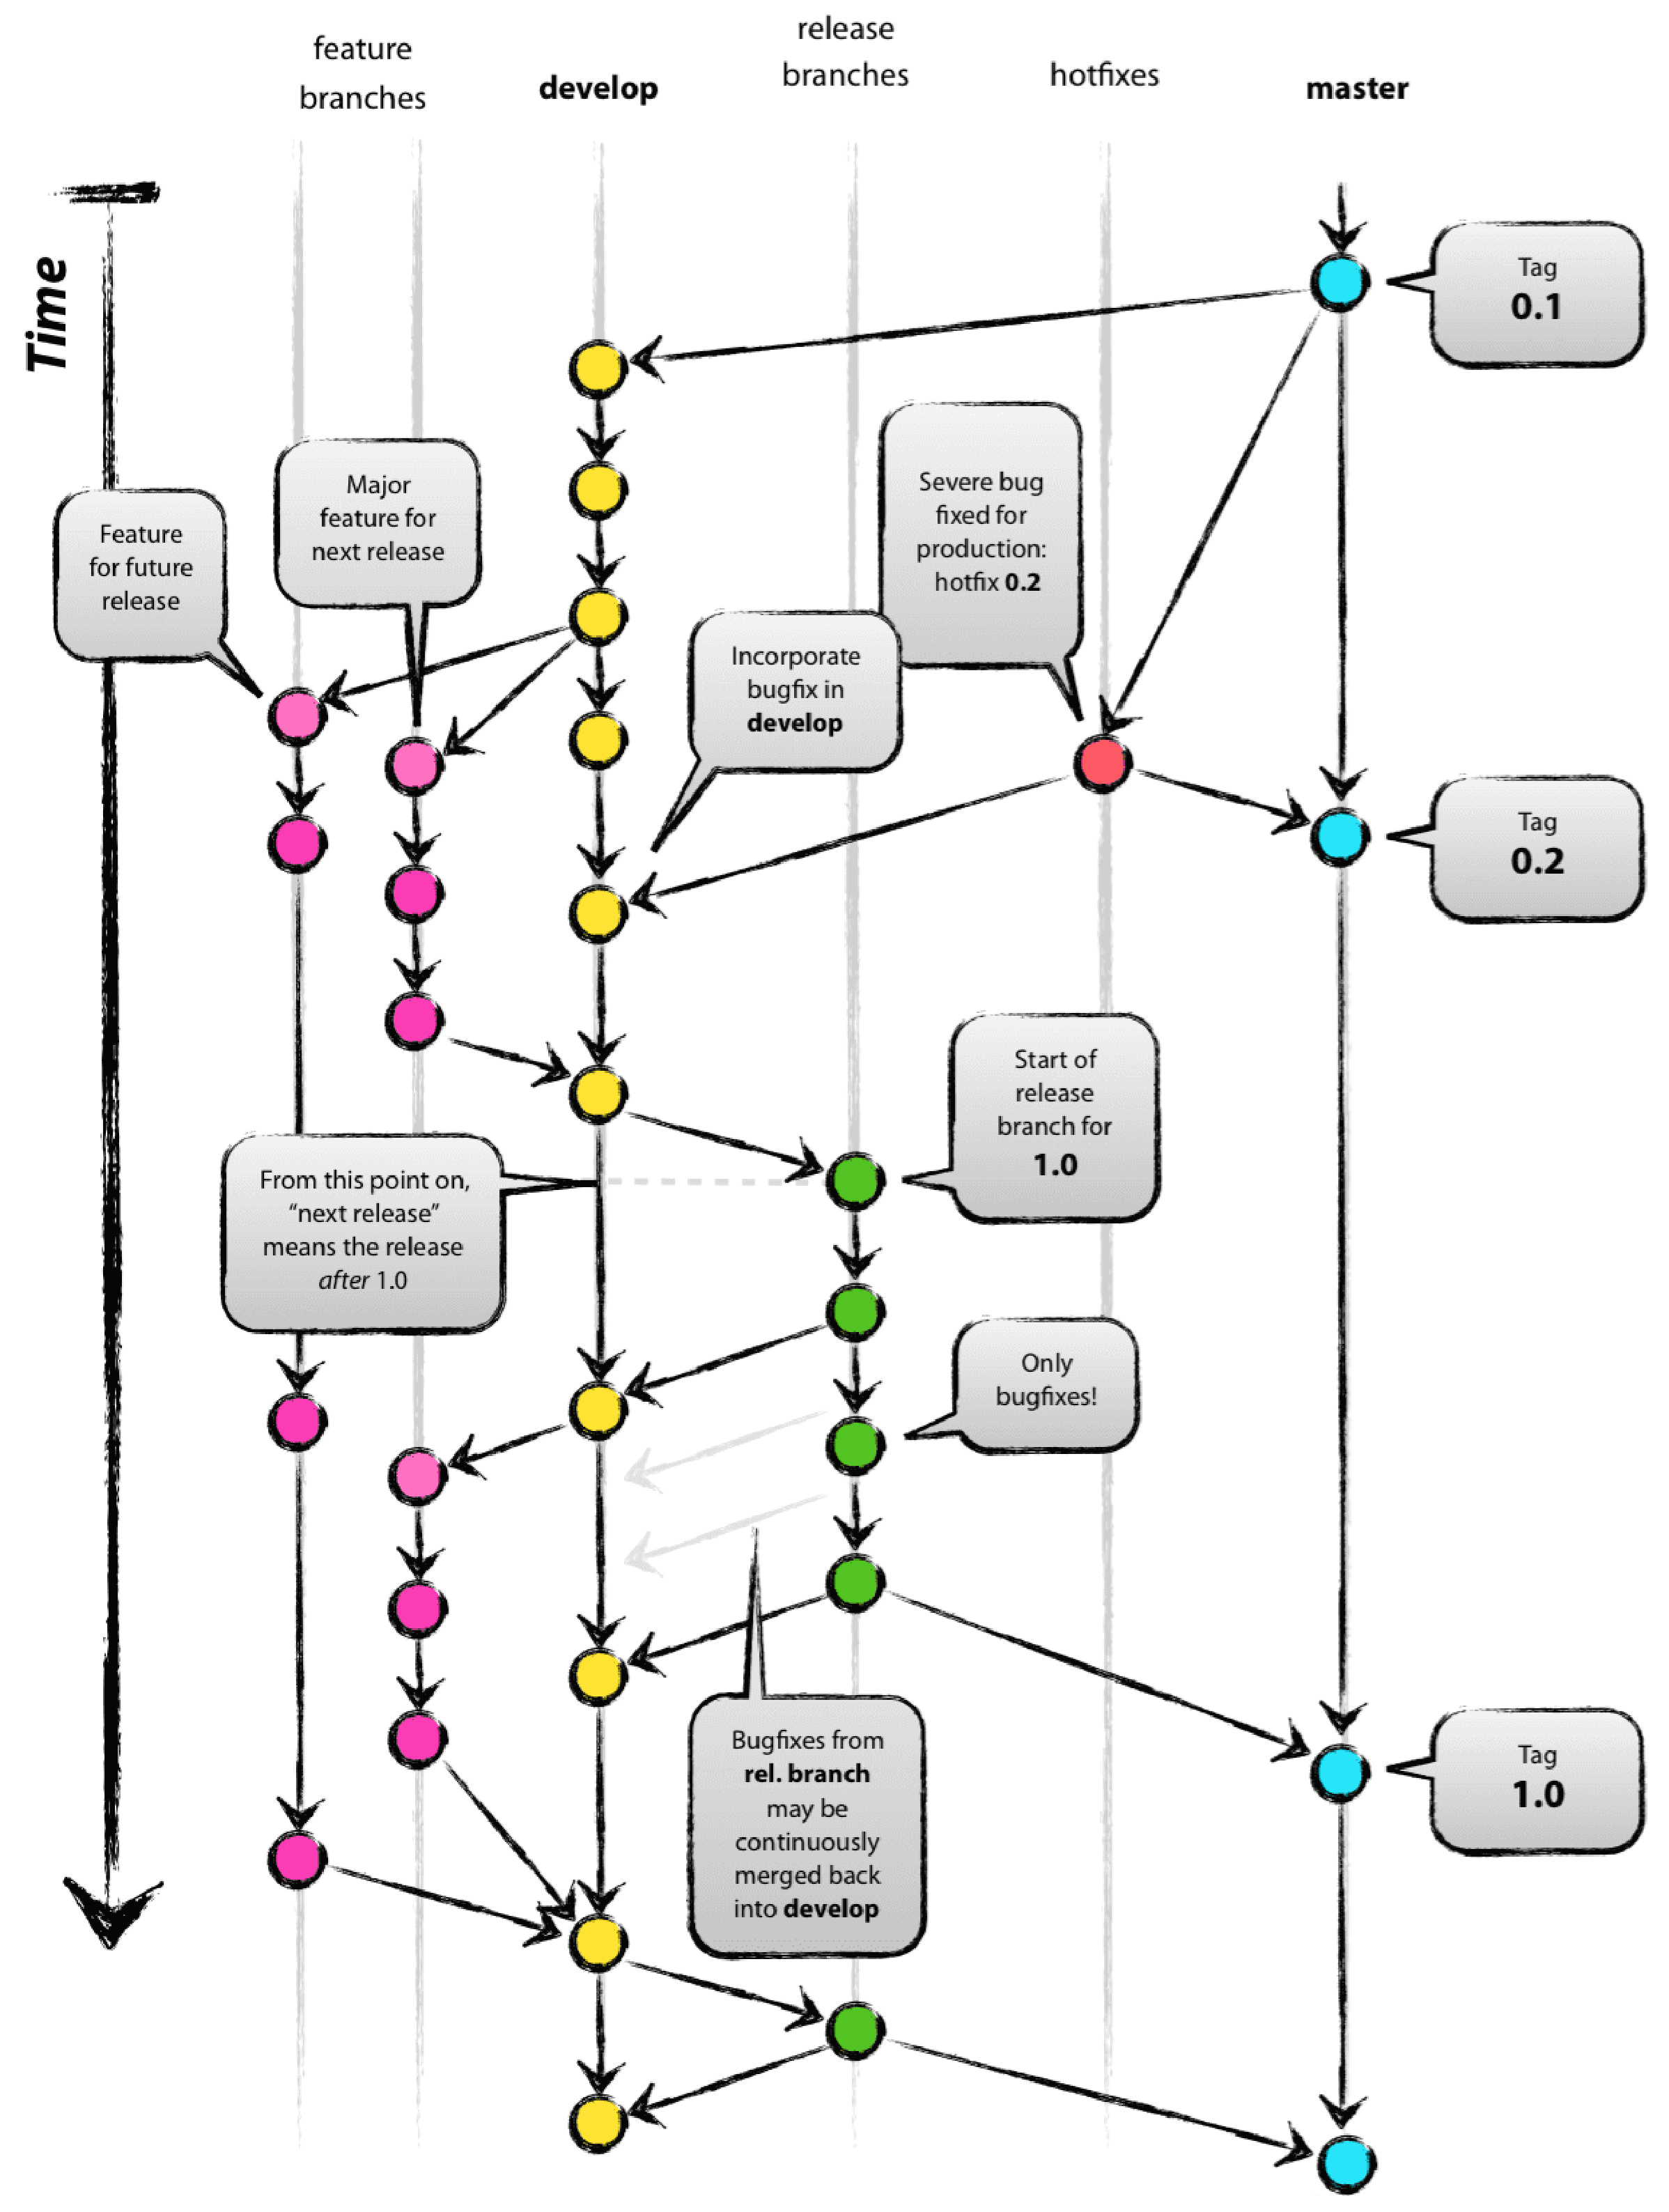
\includegraphics[width=1\linewidth]{Figure/workflow.pdf}
	\vspace{-0.3cm}
	\caption{workflow}\label{fig:workflow}
\end{figure}

\subsection{工作流与科研}
看完这张图大家是不是就明白了,APP中的版本标签V1.1,V1.2其实就是这么来的。我之所以提到工作流,主要是因为这是几乎所有大公司进行软件项目开发时采用的通用模式,这就说明解决一个问题实际上是存在一个“模式”的。作为工程硕士,我们工作的本质就是解决一些实际的工程问题,而这与公司中的工程师所做的工作并没有本质区别,因此仿照这样既有的工作模式可以使我们少犯错误。

\section{科研的模式}
我并不是所谓大牛,谈这种主题也并没有任何权威,只是摆出一些经验与感悟,图个大家乐呵。我所认为的工程类的科研模式是这样的:寻找问题 - 确定研究方法 - 提出解决方法 - 获取实验数据 - 分析处理数据 - 发表成果。
\subsection{寻找问题}
这里的问题,一般指工程类问题,与理科中那种问题(如:探究统一理论的弦论、量子力学等)并不是一类问题,因为这类研究一定是在解决人类可以接触到的直观物体中的问题,对思维大厦的构建几乎没有要求,这也使得我们的研究难度获得了大幅降低。以WPT为例,2007年MIT论文之所以具有相当高的地位并不在于首次提出了WPT(IPT的概念早在2000年就由奥克兰大学提出)并且它也并没有解决任何工程问题,相反,它的重点在于建立一个脱胎于电路以及电磁场理论的新的物理图像,这就使得这项工作具有了明确新技术以及建立新理论的双重意义。因此,我辈研究生实际上不需要对既有理论进行任何改写,仅需要对其进行理解和应用即可。

虽然避免了建立数学模型的难题,但是寻找有价值的工程问题也并不是件易事,这件事的关键在于如何\emph{快速地}获取有价值的研究方向。大家可以先自行思考,更加详细的内容请参考\cite{hopspot}。此外,比寻找问题更加重要的是对问题的重要性进行评估,这个需要很强的科研直觉,不过一般由导师代劳,这实际上也是开题时需要我们澄清的主要内容。
\subsection{确定研究方法}
对于工程问题而言,确定研究方法更多的是指采用何种数学模型,这实际上决定了后面所有工作的分析基础。电气领域的数学模型并不多,电路理论,电磁场理论,微波网络理论、状态空间、传输线理论,奇葩一点的还有日本人建立的用于解释WPT的带通滤波器理论(BFP)等。

\chapter{快速抓住研究热点}\label{hopspot}
小米总裁雷军有一句名言:“站在风口上,猪都会飞”。科技论文的核心在于创新性,而找到创新性的捷径就是跟踪科研的风口,即研究热点。然而根据自身的经验,为了培养一种对所选课题或者解决问题的判断力(或者说,一种科研直觉),需要我们对整个领域的各个研究方向建立系统认识,但研究方向却往往很难仅通过阅读论文而获得全面的快速认识,这就导致很多人并不能完全认识到自己所研究课题的价值,换句话说,认为自己的研究课题没有意义。为了解决这一问题,研究人员也提出了若干解决方案。

\section{传统方式}
词典,是语言学家针对特定语言而将常见字词按照一定的逻辑编纂起来的文本工具。科学家也有自己的词典,他们针对某一特定研究领域对热点论文进行总结归纳并提出相应见解,最终以论文的形式发表,这就是文献综述。

通过阅读文献综述,可以快速地对所关注的研究领域形成大致了解,而这也是快速抓住研究热点的传统方式。通过限定检索词可以较为有效地检索该类型的文章,对于英文文献,其检索词可以选择如下几种:
\begin{itemize}
	\item Review
	\item Challenge
	\item Survey
	\item Statement
	\item ... ...
\end{itemize}

这样,再加上一些限定词(如:WPT)就可以有效地检索出特定研究领域的文献综述。但是,这样检索出的文献往往比较松散,并且会使我们忽略一些更有价值的paper。因此有时(甚至往往)会采用辅助工具进行这项工作。

\section{辅助工具}
为了快速地了解一个领域的研究热点,仅仅通过 {\bf 关键词检索 - 论文下载 - 阅读 - 二次检索} 这类流程是不能达到“快速”的要求的,真正有效的方法是借助论文分析工具,这类工具一般有如下特点:

\begin{itemize}
	\item 可以分析大量文献间的交叉检索关系
	\item 结果可视化
	\item 多功能
\end{itemize}

常用的辅助工具有:\href{https://zhuanlan.zhihu.com/p/20902898}{HistCite Pro 2.1} 以及 \href{https://zhuanlan.zhihu.com/p/30970993}{VOSviewer}、Citespace。这两种工具的最大区别就是HistCite Pro 2.1仅支持英文文献,但VOSviewer不仅支持英文还支持中国知网导出的中文文献。笔者只用过HistCite Pro 2.1,如果读者希望对中文文献也进行处理,可以参考\href{https://www.jianshu.com/p/e20f3f1d17d8}{这个})。下面我通过若干gif对软件的使用进行介绍。
\subsection{安装}
安装就不赘述了,参考\href{https://zhuanlan.zhihu.com/p/20902898}{这里}就够了。
\subsection{导出文献}
这一步是初学者最容易出现差错的地方,这是因为HistCite Pro 2.1对源数据的格式要求非常严谨,而且它仅支持由\href{http://apps.webofknowledge.com/UA_GeneralSearch_input.do?product=UA&search_mode=GeneralSearch&SID=6DZxzSnnYfZdzYcWxLr&preferencesSaved=}{Web of Science, WOS}导出的文献格式。下面我通过Step-by-step的方式展示如何从WOS导出符合要求的格式。

第一步:选择检索{\bf 数据库}并给定检索词,一般首次使用需要我们对整个领域有一个宏观认识,因此检索词可以非常概括,比如我使用的wireless power,如图\ref{fig:1}。

\begin{figure}[!htb]
	\centering
	\animategraphics[autoplay, loop , width=0.9\linewidth]{8}{Figure//WOSsearch//10}{01}{80}
	\vspace{-0.3cm}
	\caption{WOS检索关键词:wireless power}\label{fig:1}
\end{figure}

第二步:选择正确格式,下载,如图\ref{fig:2}所示。值得注意的是,WOS仅支持一次性导出500篇文献,所以更多的文献需要多次下载,这步完成后会获得一个包含所有文献检索信息的txt文件。

\begin{figure}[!htb]
	\centering
	\animategraphics[autoplay, loop , width=0.9\linewidth]{8}{Figure//WOSdownload//00}{01}{98}
	\vspace{-0.3cm}
	\caption{WOS下载特定格式检索结果}\label{fig:2}
\end{figure}

\subsection{文献分析}
将下载获得的所有txt移动至TXT文件夹,然后打开main.exe,此时输入1并回车,软件将自动打开程序界面,接着点击gragh maker,我们就会获得文献之间的引用网络,文献由节点表示,所有的节点自上而下按照时间顺序排列,之间的引用和被引关系由连接的线条表示。修改count将对分析的文献数量进行控制,一般来说,取得大一点可以获得更多的信息,如图\ref{fig:3}所示。

\begin{figure}[!htb]
	\centering
	\animategraphics[autoplay, loop , width=0.9\linewidth]{8}{Figure//Hmaker//00}{01}{73}
	\vspace{-0.3cm}
	\caption{HistCite Pro 2.1操作}\label{fig:3}
\end{figure}


注意到,select by一栏有两个选项:LCS和GCS,LCS是Local Citation Score的缩写,代表某篇文献在本地数据集(也就是我们所下载的txt集合)的总被引次数,而GCS是Global Citation Score的缩写,代表在WOS数据库中的总被引次数。一般来说,由于本地数据集是根据我们的关键词获得的,因此LCS排名更能够反映某一学科的发展。此外,还有两个参数会出现在浏览器界面,CR和LCR,分别是Cited references和local cited references的缩写,代表对WOS数据库和本地数据库文献引用的数量。这里,CR越高(一般以50篇为标准)则表示该文献越可能是综述性文献,这样就可以方便地追根溯源,清晰地看到一个学科乃至一个领域的发展脉络,一个典型的发展脉络可以参考图\ref{fig:typical_trace}(完整版请\href{https://raw.githubusercontent.com/lonelybag/Latex_lonelybag/V1.0/Script/002_NOTE_of_MASTER/Figure/typical_trace_full.jpg}{移步})。

\begin{figure}[!htb]
	\centering
	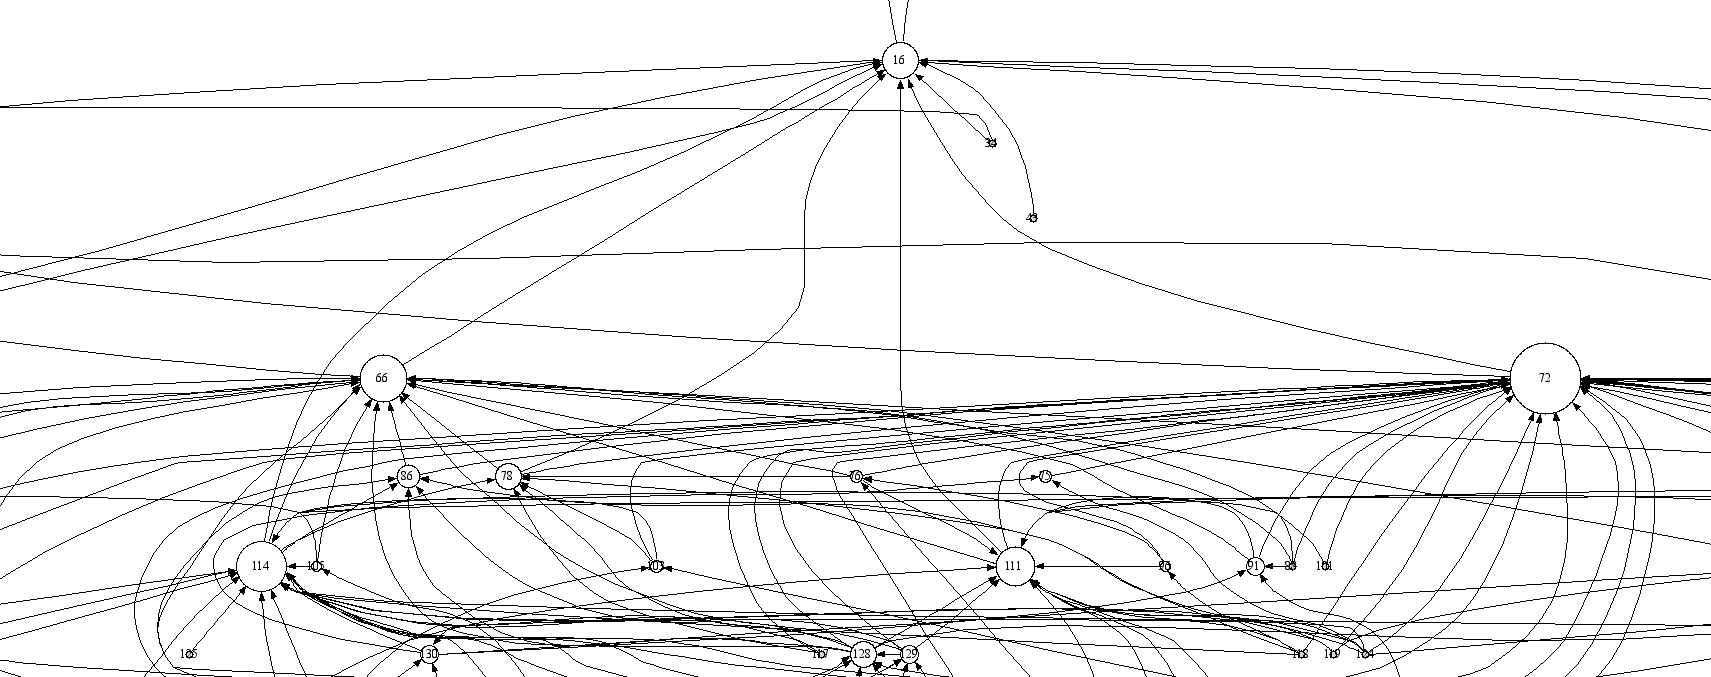
\includegraphics[width=1\linewidth]{Figure/typical_trace.JPG}
	\vspace{-0.3cm}
	\caption{一个示例}\label{fig:typical_trace}
\end{figure}

可以看出,文献16显然是这个领域的开创性论文,随着时间的推移又分裂为两个分支,接着又发展为多个分支。通过阅读关键节点论文不仅可以快速了解这个领域的发展脉络,甚至还可以看出:

\begin{itemize}
	\item 研究之初,两个小方向是经过试探却又半途而废的
	\item \href{https://raw.githubusercontent.com/lonelybag/Latex_lonelybag/V1.0/Script/002_NOTE_of_MASTER/Figure/typical_trace_full.jpg}{完整版图片}右侧出现了两个领域的交叉,这里往往是研究思路的“不老泉”
	\item \href{https://raw.githubusercontent.com/lonelybag/Latex_lonelybag/V1.0/Script/002_NOTE_of_MASTER/Figure/typical_trace_full.jpg}{完整版图片}最左侧有一个研究历程非常持久的小分支,这可能是某个专家的“独门秘籍”
	\item \href{https://raw.githubusercontent.com/lonelybag/Latex_lonelybag/V1.0/Script/002_NOTE_of_MASTER/Figure/typical_trace_full.jpg}{完整版图片}右侧还有一个完全没有关联的领域,虽然在2013年后就没有产出了,但是这并不一定意味着研究的停滞,也有可能是研究成果实现了产业化,被大佬们拿去挣钱了。。。
	\item 。。。 。。。
\end{itemize}

所以,这个方法不仅仅可以帮助我们找文献,更重要的是带给了我们关于这项研究的历史发展历程,带给了我们冰冷研究的人文情怀,我们甚至可以想象出,那位开山鼻祖级别的大佬在当时仅仅是一位年轻博士生的时候的艰苦、悲痛、遇到机遇时狂喜、受挫后的再一次站立、以及功成名就之后的平凡和悠闲。。。

因此,每一张图都可以说是一位科学家的成名史、一个领域的发展史、以及整个人类文明的历史。

所以,为什么不试试\href{https://zhuanlan.zhihu.com/p/20902898}{它}或\href{https://zhuanlan.zhihu.com/p/30970993}{它}呢?

\section{理论分析}
\subsection{为什么要建数学模型}
大到宇宙洪荒,小到亚原子领域,与人类活动相关的一切都有数学模型。那么,为什么要研究呢?我觉得其一是为了控制,其二是为了更加本质地理解现象以得到有用的结论。

\subsection{真实与仿真}
数学模型的建立,使得我们可以通过量化的方式对系统进行控制与优化,

\footnote{钱学森有一个世纪之问:“为什么中国出不了诺贝尔奖”,我自己有一个解答,不是从教育的角度,而是从国人与老外的思考方式的差异,大家有兴趣可以看看\ref{fuluA}。}

\section{实验验证}

\chapter{文献写作}
\section{写作工具}
\section{写作流程}
\section{常用软件}
在我看来,若要完成一项研究报告,我们需要完成以下(或者其中几项)任务:
\begin{itemize}
	\item 仿真
	\item 数据处理
	\item 数据可视化
	\item 算法或者设计优化流程可视化
	\item 实验系统拟物化简图
	\item 电路拓扑绘制
\end{itemize}
\subsection{仿真}
从不同理论的角度分类,可以将仿真分为电路仿真、电磁场仿真以及控制理论仿真。
所谓电路仿真,指可以对等效电路模型进行仿真的软件,一般有如下需求时需要借助该类软件:对所推导的数学模型进行正确性检验、通过快速在线地调节电路参数找创新点、
对由其他理论(如电磁场理论)获得的结论进行验证、控制算法的检验等。
常用的电路仿真软件有:Simulink、ADS或Multism、Spice、SABER、Cadence Spectre、Mentors ModelSim、\href{https://mp.weixin.qq.com/s/4AQa8VciAgzS1NZvd5tM_A}{Multisim14下载破解}、\href{https://mp.weixin.qq.com/s/qb0gipvdphj0YG8iP3IyhQ}{proteus下载破解}(可与\href{https://mp.weixin.qq.com/s/NzK8HAKlY_tXBZy8lQtfsQ}{keil下载破解}联调)、Infineon Designer、pspice(已经并入orcad)

芯片检索:alldatasheet、datasheetarchive、\href{http:\\datasheet.eeworld.com.cn}{电子工程世界}


\section{参考文献}

\chapter{未完成的事业}
有一些我认为非常重要,但是没有时间完成的事情:
\section{仿真}
\subsection{ADS}
\begin{itemize}
	\item 通过已有的数据对电路模型的特性曲线进行拟合以求取等效参数。\\
	      应用场景:1、通过几个数据点,对谐振线圈的频域曲线进行拟合,然后获得线圈的等效参数,如:分布电容,等效电感以及交流电阻。2、求取复杂电路参数,然后利用智能算法对系统参数进行设计,以优化效率、功率等。\\
	      参考:
	\item 求取频域下电流,电压以及功率。可能需要HB模块。
\end{itemize}
\subsection{Comsol}
\begin{itemize}
	\item 实现Matlab联合仿真
\end{itemize}

\subsection{Matlab}
\begin{itemize}
	\item 实现C MEX语言编译
	\item 实现Simulink控制算法的直接生成以驱动硬件电路
\end{itemize}

\section{文献写作}
\subsection{Latex}
\begin{itemize}
	\item 控制表格中的字体大小
	\item 控制浮动体的位置
	\item 坏箱的修复
	\item 看懂并修改cls文件
	\item 看懂并修改bst文件
	\item 写一份符合学校要求的模板cls文件(需要多人协作)
\end{itemize}

\section{绘图}
\begin{itemize}
	\item 3DSMAX 渲染器的设置
	\item Rhino 渲染器的设置
	\item 找到高效美观并且符合标准的电路图绘制软件
	\item 找到高效美观并且符合标准的流程图绘制软件
	\item 学会Adobe Illustrator
\end{itemize}


\chapter{上帝说:要有神器}
积累了一些常用的工具类软件和网站,我只用过其中的一部分,另一部分是还没有时间尝试的,\underline{下划线}表示使用过的软件(网址没有标记,都用过)。

\section{基本}
\subsection{杀毒+垃圾整理+系统优化}
\begin{itemize}
	\item \underline{\textit{\href{https://www.huorong.cn}{火绒}}}\quad 免费
	\item \underline{\textit{\href{http://ccleaner.soft88.com}{ccleaner}}}\quad 基础版免费
	\item \href{https://bitsum.com}{Process Lasso}\quad 用于优化系统进程,提高运行速度,收费
	\item \href{https://fastcopy.jp/en/}{FastCopy}\quad 文件复制加速软件,免费
	\item \underline{\textit{\href{https://www.listary.com}{Listery}}}\quad 用于快速搜索文件,免费
	\item \href{http://www.disktool.cn/download.html}{傲梅分区助手}\quad 用于分区,免费
	\item \href{http://www.bandisoft.com}{Bandizip}\quad 据说是第二好用的压缩软件,免费
\end{itemize}

\subsection{卸载类}
\begin{itemize}
	\item \href{https://geekuninstaller.com}{Geek}\quad 免费
	\item \underline{\textit{\href{https://www.revouninstaller.com/}{Revo Uninstaller Pro}}}\quad 收费
	\item \underline{\textit{\href{https://lockhunter.com}{lockhunter}}}\quad 用于删除时出现该文件正在占用,3M,免费
	\item
\end{itemize}

\subsection{下载}
\begin{itemize}
	\item \href{http://jdownloader.org/jdownloader2}{JDownloader2}
	\item \href{http://xdman.sourceforge.net}{Xtreme Download Manager}\quad 36M,免费
	\item \href{https://www.freedownloadmanager.org/}{FDM}\quad 48.7M,免费
	\item \href{https://webtorrent.io}{磁力在线播放}
	\item \href{https://send-anywhere.com}{Send Anywhere}\quad 设备之间的分享
	\item 百度网盘满速下载,微信关注 科研利器
\end{itemize}

\subsection{制作文档类}
\begin{itemize}
	\item GIF录屏:\underline{\textit{\href{https://www.cockos.com/licecap/}{LICEcap}}}\quad 230kb免费、\href{https://www.screentogif.com/?l=zh_cn}{ScreenToGif}\quad 2M免费、\href{https://ocam.en.softonic.com}{Ocam}\quad 10Mb免费
	\item Gif转换为图片:\underline{\textit{\href{https://ulead-gif-animator.jaleco.com}{Ulead GIF Animator}}}\quad 免费
	\item PDF转换为矢量图片:\underline{\textit{\href{https://inkscape.org}{Inkscape}}}\quad 免费
	\item \underline{\textit{\href{https://code.visualstudio.com}{VScode}}}\quad 免费
	\item \underline{\textit{\href{https://mirrors.tuna.tsinghua.edu.cn/CTAN/systems/texlive/Images/}{Texlive}}}\quad 免费
	\item 截屏:\underline{\textit{\href{http://www.faststone.org/FSCaptureDetail.htm}{FastStone Capture}}}\quad 收费、\href{https://www.snipaste.com}{Snipaste}\quad 免费
	\item 快速浏览:\href{https://pooi.moe/QuickLook/}{QuickLook}\quad 免费、\href{http://1218.io}{seer}\quad 收费
	\item \href{https://otp.landian.vip/zh-cn/}{office365}
	\item \href{http://www.dayanzai.me/infixpro-pdf-editor.html}{InfixPro PDF Editor}\quad 修改PDF
\end{itemize}

\subsection{Chrome插件类}
\begin{itemize}
	\item \underline{\textit{\href{https://greasyfork.org/zh-CN}{油猴脚本}}}\quad 免费
	\item VPN:就去加速(官网已被墙)
	\item \underline{\textit{\href{http://listen1.github.io/listen1/}{Listen1}}}\quad 最好用的在线音乐播放器,免费
	\item \href{https://kopernio.com}{Kopernio}\quad 免费获取论文,免费
\end{itemize}

\subsection{常用网站}
\begin{itemize}
	\item 软件下载
	      \begin{itemize}
		      \item \href{https://www.3d66.com/popsoft_26.html}{软件下载}\quad 包括但不限于:3DSMAX,AutoCAD,PS,Rhino,Maya,AI。。。
		      \item \href{https://www.appinn.com/category/windows/}{小众软件}
		      \item \href{https://filehippo.com/zh/}{国际类软件网站}
	      \end{itemize}
	\item Git
	      \begin{itemize}
		      \item \href{http://gitbook.liuhui998.com/index.html}{gitbook}
		      \item \href{https://learngitbranching.js.org/?demo}{动画学习Git}
	      \end{itemize}
	\item 在线工具
	      \begin{itemize}
		      \item \href{https://tool.lu}{程序员的工具箱}
		      \item \href{https://cloudconvert.com/gif-to-mp4}{Gif2MP4}
		      \item \href{https://cn.office-converter.com/FIG-to-EPS}{Fig2EPS}
		      \item \href{http://www.ytube.win}{下载youtube视频}\quad 缺点是不带字幕
		      \item \href{https://www.slant.co}{帮助我们做决策}
		      \item \href{https://www.photopea.com}{在线PS}
		      \item \href{https://uzer.me/u/signin}{在线office,PS,AI,MATLAB等}
		      \item \href{https://bigjpg.com}{无损放大图片}
		      \item \href{https://www.remove.bg}{自动抠图}
	      \end{itemize}
	\item 在线学习
	      \begin{itemize}
		      \item \href{http://www.xuexiniu.com/forum.php?mod=forumdisplay&fid=102&filter=typeid&typeid=1}{犀牛技巧}
		      \item \href{http://www.pythontutor.com}{python代码在内存中是如何执行的}
		      \item \href{https://algorithm-visualizer.org}{算法运行可视化}
	      \end{itemize}
\end{itemize}

\section{论文写作}
\subsection{制作文档类}
\begin{itemize}
	\item \underline{\textit{\href{https://mirrors.tuna.tsinghua.edu.cn/CTAN/systems/texlive/Images/}{Texlive}}}\quad 免费
	\item 思维导图:\href{https://mubu.com}{幕布}\quad 34Mb,免费
	\item 截屏:\underline{\textit{\href{http://www.faststone.org/FSCaptureDetail.htm}{FastStone Capture}}}\quad 收费、\href{https://www.snipaste.com}{Snipaste}\quad 免费
	\item \href{https://picpick.app/zh/}{PicPickp}\quad 屏幕取色
	\item \href{https://ditto-cp.sourceforge.io}{Ditto}\quad 剪切板神器,免费
\end{itemize}

\subsection{Chrome插件类}
\begin{itemize}
	\item \href{https://kopernio.com}{Kopernio}\quad 免费获取论文,免费
\end{itemize}

\subsection{英语写作}
\begin{itemize}
	\item 英语语法检查 \href{https://languagetool.org}{LanguageTool}、\underline{\textit{\href{https://www.grammarcheck.net}{grammercheck}}}、\href{https://www.scribens.com}{scribens}、\href{https://www.grammarly.com}{grammerly}、\href{https://www.nounplus.net}{nounplus}
	\item 查单词搭配等等 \underline{\textit{\href{https://www.english-corpora.org/coca/}{ Corpus of Contemporary American English}}}、\href{https://www.lintcode.com}{linggle}
	\item 近义词 \underline{\textit{\href{https://www.thesaurus.com}{theasurus}}}
\end{itemize}

\subsection{科研常用网站}
\begin{itemize}
	\item 文献写作
	      \begin{itemize}
		      \item \href{http://www.latexstudio.net/archives/6888.html}{GB/T7714-2015参考文献格式}\quad 毕业论文参考文献,自动生成
		      \item \href{https://www.processon.com/login;jsessionid=022BCDCA031DD3C240BE7FD87D942F03.jvm1?backUrl=/diagraming/5be7a513e4b0d74dc539976e}{流程图}
		      \item Latex相关:
		            \begin{itemize}
			            \item \href{http://detexify.kirelabs.org/classify.html}{手写LaTeX符号}
			            \item \href{http://www.jabref.org}{JabRef}\quad 开源的文献管理软件
			            \item \href{http://www.latexstudio.net/archives/6992.html}{Excel2Latex}
			            \item \href{http://www.ursoswald.ch/metapost/introduction.html}{MetaPOST}\quad 矢量绘图软件
			            \item \href{http://www.gnuplot.info}{Gnuplot}\quad 绘制矢量数据图
			            \item \href{https://www.tablesgenerator.com/#}{在线绘制表格}
			            \item \href{http://math.ecnu.edu.cn/~jypan/Teaching/Latex/}{LaTeX 科技排版}
			            \item \href{http://www.latexstudio.net/}{latex开源小屋}
			            \item \href{https://github.com/latexstudio}{Latex中文社区Github}
			            \item \href{https://www.overleaf.com/login}{在线编辑器1}、\href{http://www.math.org.cn/tex/index.html}{在线编辑器2}
			            \item \href{http://www.bakoma-tex.com}{一个我认为完美的编辑器}\quad 缺点:收费
		            \end{itemize}
	      \end{itemize}
	\item 绘图
	      \begin{itemize}
		      \item \href{https://www.photopea.com}{在线PS}
		      \item \href{https://uzer.me/u/signin}{在线office,PS,AI,MATLAB等}
		      \item \href{https://bigjpg.com}{无损放大图片}
		      \item \href{https://www.remove.bg}{自动抠图}
		      \item 思维导图:\href{http://naotu.baidu.com/file/97d9cd5ca30672903a3e3321e62c6ed8}{百度脑图}、\href{https://www.xmind.net/}{Xmind}
		      \item \href{http://www.colorhunter.com}{Color Hunter}\quad 配色
		      \item \href{https://color.adobe.com/zh/create/color-wheel/?base=2&rule=Analogous&selected=0&name=我的%20Color%20主題&mode=rgb&rgbvalues=1,0.8549019607843137,0.598371339694025,0.91,0.33228399543185755,0.04550000000000004,1,0,0,0.8452221384131547,0.04550000000000004,0.91,0.3394492552539419,0.050000000000000044,1&swatchOrder=0,1,2,3,4}{Adobe Color CC}
		      \item
	      \end{itemize}
	\item 学习类
	      \begin{itemize}
		      \item \href{https://www.52pojie.cn/thread-716675-1-1.html}{一个电路仿真APP}\quad 特点是,可以看到电流
		      \item \href{https://mm.edrawsoft.cn/map.html?obj=wxoa3v5wBLcpmgCifx59_Uzk5X4qHU/Personal/未命名文件.emmx}{思维导图}更专业一点
		      \item \href{https://ankiweb.net/shared/decks/}{记忆神器}
	      \end{itemize}
	\item 算法以及神经网络
	      \begin{itemize}
		      \item \href{https://leetcode.com}{Leetcode}以及\href{https://www.lintcode.com/zh-cn/accounts/signup/}{lintcode} 代码训练平台
		      \item \href{https://algorithm-visualizer.org}{算法运行可视化}
		      \item \href{https://www.stateoftheart.ai}{MIT整理的关于神经网络的论文}
		      \item \href{https://github.com/lonelybag/pwc}{神经网络论文以及源代码}\quad 万能的GitHub
	      \end{itemize}
\end{itemize}

\subsection{绘图}
\begin{itemize}
	\item 电路图
	      \begin{itemize}
		      \item Viso
		      \item Latex
		      \item Python
		      \item
	      \end{itemize}
	\item 流程图:
	      \begin{itemize}
		      \item
	      \end{itemize}
	\item 统计数据函数图:
	      \begin{itemize}
		      \item Origin
		      \item Sigmaplot
		      \item Graphpad
		      \item geogebra(开源)
		      \item SPSS
		      \item NVivo
	      \end{itemize}
	\item 2D 图形
	      \begin{itemize}
		      \item Photoshop
		      \item Adobe Illustrator
		      \item \href{https://affinity.serif.com/zh-cn/designer/}{affinity designer}
	      \end{itemize}
	\item 3D 拟物图
	      \begin{itemize}
		      \item C4D
		      \item 3ds MAX
	      \end{itemize}
\end{itemize}

\section{其他}
\begin{itemize}
	\item Send Anywhere
	\item \href{https://www.scimagojr.com}{SCI期刊}
	\item \href{http://libgen.io}{免费专业书籍}
\end{itemize}

\section{最小配置}
在此给出一个我常用的\emph{最小基础配置}:
\begin{itemize}
	\item 杀毒软件:\href{https://www.huorong.cn}{火绒}
	\item 卸载软件:\href{http://www.xue51.com/soft/11977.html}{Revo Uninstaller Pro}
	\item 文档撰写:\href{https://mirrors.tuna.tsinghua.edu.cn/CTAN/systems/texlive/Images/}{\LaTeX} 和 WORD
	\item PDF阅读:\href{https://www.tracker-software.com/product/pdf-xchange-editor}{PDF-XChange Editor}
	\item 视频播放:\href{http://potplayer.daum.net/?lang=zh_CN}{PotPlayer}
	\item 文件搜索:\href{https://www.listary.com}{Listery}
	\item 撸代码: \href{https://code.visualstudio.com}{VScode}
	\item 版本管理+团队协作:\href{https://git-scm.com}{Git}
\end{itemize}

\emph{最小科研配置}:
\begin{itemize}
	\item 计算与仿真:
	      \begin{itemize}
		      \item 数值计算:Matlab、Mathematica
		      \item 电路仿真:ADS、Simulink
		      \item 电磁场仿真:Comsol
	      \end{itemize}
	\item 文档撰写:
	      \begin{itemize}
		      \item Latex
		      \item Endnote
		      \item \href{https://zhuanlan.zhihu.com/p/20902898}{HistCite Pro 2.1}
	      \end{itemize}
\end{itemize}



\backmatter
\chapter*{跋}\addcontentsline{toc}{chapter⟩}{跋}
讲几个事例作为结束。

\subsection*{热爱}
时常有人问我:“你怎么会有时间去学那么多东西的?”。其实很简单,因为热爱。

\subsection*{持久的输出}
知乎上有一个问题,苹果公司有哪些黑科技?其中一个回答的答案是iPhone一代。2007年1月,苹果公司发布了被后人称为“重新定义了手机”的iPhone一代,自此开始了长达十年的封神之路。作为历史上市值第一个超过万亿美元的科技公司,它的成功也让很多人萌发了试图复制这一商业成功的欲望,当然他们并未成功,因为十年后的今天苹果依然是第一。很多人将苹果的成功归功于乔布斯,这种想法其实很愚蠢。那么到底是什么造就了它的成功呢?

如果大家读过《乔布斯传》就会了解到,2007年发布的iphone一代,其实早在5年前就已经开始准备了。那就是2002年,还是各种翻盖、滑盖、旋转盖手机迭起的风云时代。。。

我们输的不冤枉。对手感觉到的“黑科技”,其实对自己不过是孕育和必然。

\subsection*{人为什么活着?}
为了心中的梦想。

\vspace{2cm}
总结起来就是三句话:试着让内心去做决策,时刻雕琢自己以及捍卫梦想。

\hspace{4cm}\\
\noindent2019毕业前夕\\
于天津工业大学 \quad 电气学院







\chapter*{附录 A}\addcontentsline{toc}{chapter⟩}{附录 A}\label{fuluA}
如果大家看过《降临》这部电影就会了解,语言决定了(或者反映了)一个人的思考方式,电影中的外星人具有非线性的高维语言能力,没有时间空间的线性概念,这也是电影中人类语言学家不能理解外星人文字的症结。我们可以仿照着看一下汉语与英语的差别,如表\ref{tab:compareCandE}:

\begin{table}[!htb]
	\renewcommand{\arraystretch}{1.3} %可以让行显得更加宽敞
	\caption{中英对比}\label{tab:compareCandE}
	\centering
	\vspace{0.2cm}
	\resizebox{0.3\columnwidth}{!}{
		\begin{tabular}{ccc} % 通过添加 | 来表示是否需要绘制竖线
			\hline  % 在表格最上方绘制横线
			对比       & 汉语 & 英语 \\
			\hline  %在第一行和第二行之间绘制横线
			奇怪的量词 & 少   & 多   \\
			感情色彩   & 委婉 & 直接 \\
			时态       & 无   & 有   \\
			\hline % 在表格最下方绘制横线
		\end{tabular}
	}
\end{table}

可以看出,中国人的语言是弱化量词而强化情感的,我们作画作诗也是这样,总是注重写意而避免写实,描述人与自然的关系的时候也总是旁击侧引,生怕赏画吟诗的人一眼就看穿作者的心思。但是外国人并不是这样,他们致力于用最简练最准确的语言描述事物,生怕哪个词读者不明白而影响了本意。

从牛顿时代开始,这个社会的生产力就是纯粹的科技力量了,而科技恰恰要求的是高精度:优化算法是为了更加精确和更加快速地求解方程、学习CAD是为了更加精确地描述事物的几何特性、发明电子计算机是为了更加精确地制导。。。看到这里,不知道读者是否明白了我的意思。

\end{document}
